\section{2008 - PHYSICS 2A  ALTERNATIVE A PRACTICAL}

\begin{enumerate}
\item[1.] The aim of this experiment is to investigate whether string A obeys Hooke's law.

\begin{center}
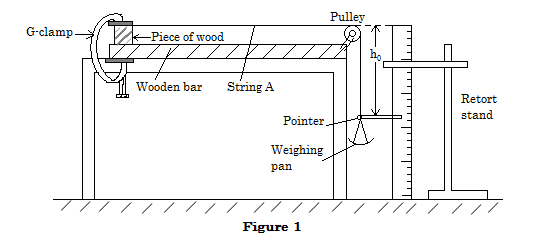
\includegraphics[width=15cm]{./img/2008-1-alt.png}
\end{center}

Proceed as follows:\\[6pt]

Clamp string A at one end, attach a weighing pan at the other end and a pointer to give a reading on a scale as shown in figure 1 above.\\[6pt]

Measure the height, $h_0$ when the pan is empty.\\[6pt]

Place 50 g mass on the pan and record the new height $h$ indicated by the pointer.\\[6pt]

Add another 50 g mass each time up to 300 g, and record the corresponding values of $h$ for added mass.

\begin{enumerate}
\item[(a)] Tabulate your results as shown in the table below.
\item[] $h_0 = $ \begin{tabular}{p{1.5cm}}
\\ \hline
\end{tabular} cm.\\[10pt]

\begin{tabular}{|c|c|c|c|c} \hline
Mass, $m$ (g) & Height, $h$ (cm) & Extension ($h - h_0$) & Stretching \\
&&(cm)&force, $F$ (N) \\ \hline
50&&& \\ 
100&&& \\ 
150&&& \\ 
200&&& \\ 
250&&& \\ 
300&&& \\ \hline
\end{tabular}\\[10pt]
\item[(b)] Plot a graph of force $F$ (N) against extension (cm).
\item[(c)] From the graph find the
\begin{enumerate}
\item[(i)] slope, K of the graph.
\item[(ii)] extension caused by a mass of 180 g.
\end{enumerate}
\item[(d)] Deduce whether string A obeys Hooke's law.
\item[(e)] State the law. \hfill \textbf{(25 marks)}
\end{enumerate}
\end{enumerate}

\begin{enumerate}
\item[2.] You are provided with a glass block, four sheets of drawing paper, four optical pins (or office pins) and a drawing board.\\[6pt]

Proceed as follows:\\[6pt]

Place the glass block flat on the drawing paper fixed to the drawing board and with a sharp pencil, draw its outline.

\begin{center}
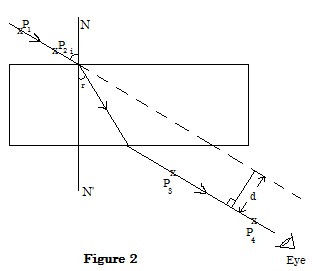
\includegraphics[width=9cm]{./img/2008-2-alt.png}
\end{center}

Remove the glass block and draw a normal NN' to the longer edge of the block (see fig. 2).\\
Draw a line making an angle of incidence ($i$) of 30$^\circ$. Stick two vertical pins P$_1$ and P$_2$ on this line. Replace the glass block. Stick two more pins P$_3$ and P$_4$ on the other side of the block so that they appear to be in the same straight line with the images of pins P$_1$ and P$_2$ as seen through the block.\\
Remove the block and draw the complete path of the ray entering and leaving the block.\\
Measure the angle of refraction ($r$).\\[6pt]

Produce the incident ray as shown in fig. 2 and measure the perpendicular distance ($d$) between the incident ray and the emergent ray.\\
Repeat this procedure for angles of incidence of $40^\circ$, $50^\circ$, $60^\circ$ and $70^\circ$. In each case draw the block again on a fresh part of the paper.
\begin{enumerate}
\item[(a)] Record your results in a table as follows:
\begin{tabular}{|p{0.15\textwidth}|p{0.15\textwidth}|p{0.15\textwidth}|p{0.15\textwidth}|p{0.15\textwidth}|} \hline
\multicolumn{1}{|c|}{$i^\circ$} & \multicolumn{1}{c|}{$r^\circ$} & \multicolumn{1}{c|}{$d$ (cm)} & \multicolumn{1}{c|}{$d\cos{r}$ (cm)} & \multicolumn{1}{c|}{$\sin{(i-r)}$} \\ \hline
\multicolumn{1}{|c|}{30}&&&& \\
\multicolumn{1}{|c|}{40}&&&& \\
\multicolumn{1}{|c|}{50}&&&& \\
\multicolumn{1}{|c|}{60}&&&& \\
\multicolumn{1}{|c|}{70}&&&& \\ \hline
\end{tabular}\\[10pt]
\item[(b)] Plot a graph of $d \cos{r}$ (vertical axis) against $\sin{(i - r)}$ (horizontal axis).
\item[(c)] Find the gradient of the graph.
\item[(d)] Measure the width of the glass block.
\item[(e)] How is the gradient related to the with of the glass block?
\item[] NB: Hand in your diagrams together with your answer booklet. \hfill \textbf{(25 marks)}
\end{enumerate}
\end{enumerate}

\begin{enumerate}
\item[3.] The aim of this experiment is to determine the resistance of a wire W.\\
Proceed as follows:
\begin{enumerate}
\item[(a)] Connect in series the full length of wire W of unknown resistance, battery B (3 V), a switch K, a rheostat Rh of a few ohms and an ammeter A of $0 - 1$ A.\\
Connect the voltmeter V of $0 - 3$ V across W. Check that the +ve side of the ammeter A and the +ve side of the voltmeter V are both on the +ve side of the battery B.
\item[(b)] Switch on the current. Adjust the rheostat to obtain five widely different values of $V$ and corresponding values of current $I$.
\item[(c)] Tabulate your results as follows:\\[10pt]
\begin{tabular}{|p{4cm}|p{4cm}|} \hline
\multicolumn{1}{|c|}{Potential difference} & \multicolumn{1}{c|}{Current $I$ (amperes)} \\
\multicolumn{1}{|c|}{$V$ (volts)} & \\ \hline
& \\ 
& \\ 
& \\ \hline
\end{tabular}
\item[(d)]
\begin{enumerate}
\item[(i)] Draw a circuit diagram.
\item[(ii)] Plot a graph of potential difference $V$ against current $I$.
\item[(iii)] Find the slope of the graph.
\item[(iv)] Determine the resistance of the wire W.
\item[(v)] Mention \textbf{two (2)} main precautions to be taken in this experiment.
\end{enumerate}
\end{enumerate}
\end{enumerate}
\flushright \textbf{(25 marks)}
\flushleft